\documentclass[11pt]{article}
%Gummi|065|=)
\title{\textbf{Meccano nonagon}}
\author{https://github.com/heptagons/meccano/nona}
\date{}

\usepackage{amsmath}
\usepackage[pdftex]{graphicx}

\begin{document}

\maketitle

\section{Meccano regular nonagon}

\begin{figure}
\centering
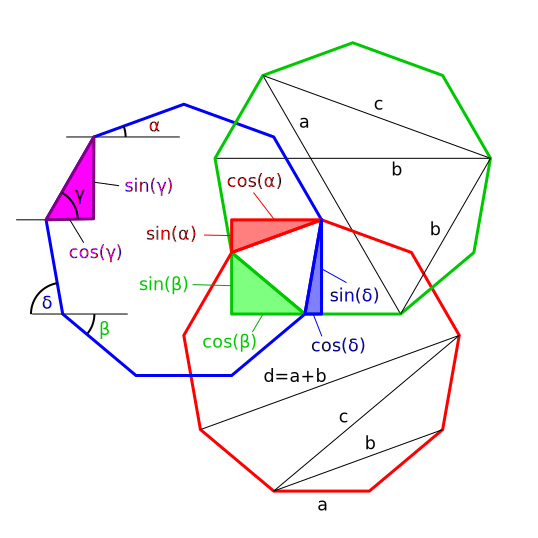
\includegraphics[scale=0.75]{figs/3nonagons}
\caption{Three regular nonagons connected by an equilateral triangle.
We note four angles in the figure $A$, $B$, $C$ and $D$.}
\label{fig:1}
\end{figure}

Figure \ref{fig:1} shows three regular nonagons connected by an equilateral 
triangle. Four angles appear orthogonally in any regular nonagon:
\begin{align*}
A &= \pi/9 = 20^{\circ} \\
B &= 2\pi/9 = 40^{\circ} \\
C &= 3\pi/9 = 60^{\circ} \\
D &= 4\pi/9 = 80^{\circ}
\end{align*}

The relations of angle $D$ are those of equilateral triangle:
\begin{align*}
\cos{D} &= -\frac{1}{2}\\
\sin{D} &= \frac{\sqrt{3}}{2}
\end{align*}

From the figure \ref{fig:1}, cosines of angles $A$, $B$ and $C$ are related as:
\begin{align*}
\cos{C} &= \cos{A} - \cos{B}
\end{align*}

Since by definition $C=4A$ and $B=2A$ previous equation converts into:
\begin{align*}
\cos{4A} &= \cos{A} - \cos{2A}
\end{align*}

Previous cosines equation solves this cubic equation:
\begin{align*}
8x^3 - 6x - 1 &= 0\\
x^3 - \frac{3x}{4} - \frac{1}{8} &= 0\\
x_1 &= +\cos{A} \approx +0.939692 \\
x_2 &= -\cos{B} \approx -0.766044 \\
x_3 &= -\cos{C} \approx -0.173648
\end{align*}

More cosines relations are:
\begin{align*}
\cos{A}\cos{B}\cos{C} &= \frac{1}{8} \\
\cos^2{A} + \cos^2{B} + cos^2{C} &= \frac{3}{2}
\end{align*}

From the figure \ref{fig:1}, sines of angles $A$, $B$ and $C$ are related as:
\begin{align*}
\sin{C} &= \sin{B} + \sin{A}
\end{align*}

Since by definition $C=4A$ and $B=2A$ previous equation converts into:
\begin{align*}
\sin{4A} &= \sin{2A} + \sin{A}
\end{align*}

Last equation solves this cubic equation:
\begin{align*}
y^3 - \frac{3y}{4} - \frac{3}{8} &= 0\\
y_1 &= -\sin{A} \approx -0.342020\\
y_2 &= -\sin{B} \approx -0.642787\\
y_3 &= +\sin{C} \approx +0.984807
\end{align*}

More sines relations of angles $A$, $B$ and $C$ are:
\begin{align*}
\sin{A}\sin{B}\sin{C} &= \frac{\sqrt{3}}{8}\\
\sin^2{A} + \sin^2{B} + \sin^2{C} &= \frac{3}{2}
\end{align*}

Cosines and sines relations are:
\begin{align*}
\cos{A}\cos{B} - \sin{A}\sin{B} &= \frac{1}{2}\\
\frac{1}{\cos{C}} -\frac{\sqrt{3}}{\sin{C}} &= 4\\
\tan{C} - 4\sin{C} &= \sqrt{3}
\end{align*}

\end{document}
